

\begin{figure}[t]
  \centering
  \begin{minipage}{0.49\textwidth}
    \subfloat[$(Q_e$]{
      \lstinputlisting[
        basicstyle=\scriptsize\sffamily,
        language=sparql,
        numbers=none,
        columns=fixed,
        showstringspaces=false]{
          figures/query-q1-j2-no-star.rq
        }
      \label{fig:q1-j2-1hop}
    } \\
    % \subfloat[$(Q_1^{J_2})^{1..2}$]{
    %   \lstinputlisting[
    %     basicstyle=\scriptsize\sffamily,
    %     language=sparql,
    %     numbers=none,
    %     columns=fixed,
    %     showstringspaces=false]{
    %       figures/query-q1-j2-2hop.rq
    %     }
    %   \label{fig:q1-j2-2hop}
    % }
  \end{minipage}
  \hfill
  \begin{minipage}{0.50\textwidth}
    \subfloat[RDF graph $G_1$]{
      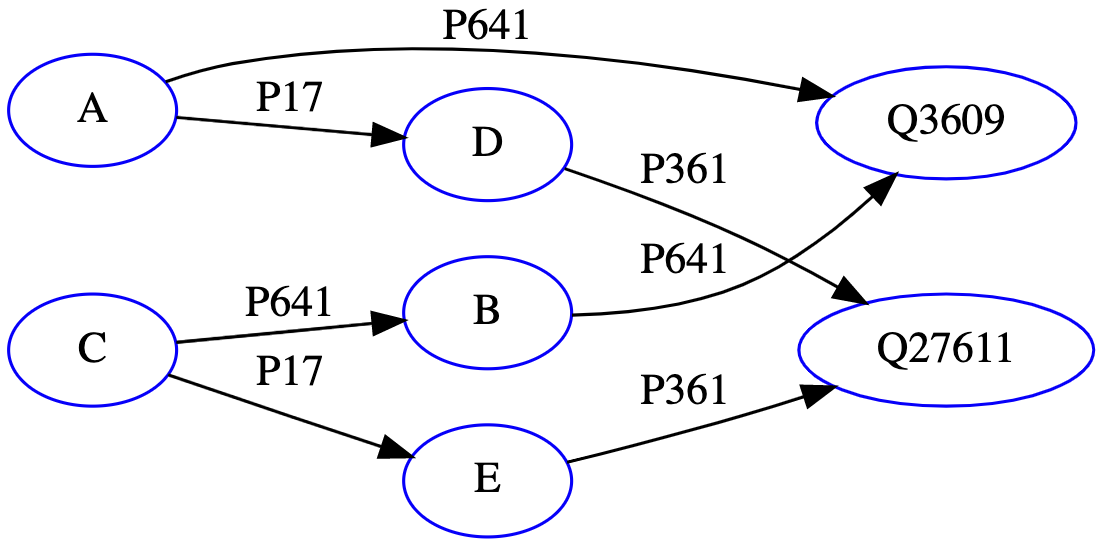
\includegraphics[width=\textwidth]{figures/graph-g1.png}
    }
  \end{minipage}
  \caption{
    query $Q_e$  evaluated on RDF graph $G_1$.
  }
  \label{fig:random_walks_example}
\end{figure}



\section{\NAME}


\paragraph{Sampling principles}


Let $Q$ be a SPARQL conjunctive query, and $J = \langle tp_1, ..., tp_n \rangle$ be
the join order used to perform random walks. A random walk
$\gamma_i = \langle t_1, ..., t_n\rangle$ is computed over
an RDF graph $G$ by randomly picking $t_1$ in $\llbracket tp_1 \rrbracket_G$,
and each subsequent $t_i$ ($i > 1$) in $\llbracket t_{i-1} \bowtie tp_i \rrbracket_G$.
Once computed, the cardinality of $Q$ is estimated as the inverse probability
of sampling $\gamma_i$, i.e. $P(\gamma_i)^{-1}$, with $P(\gamma_i) = |\llbracket tp_1 \rrbracket_G|^{-1} \prod_{i=2}^{n}
|\llbracket t_{i-1} \bowtie tp_i \rrbracket_G|^{-1}$.

For instance, let us consider the query $Q_e$ and the RDF graph $G_1$
depicted in Figure~\ref{fig:random_walks_example}. Following the join order $tp_3,tp_2,tp_1$, the random walk 
$\gamma_1$ is computed as follow:

% \begin{center}
  \begin{small}
    \begin{tabular}{l|lll}
      $tp_3$ & draw  $t_1$ &$= (\textbf{A}, P641, Q3609)$ & $\in \llbracket (?x1, P641, Q3609) \rrbracket_{G_1}$ \\
      $tp_2$ & draw  $t_2$ &$= (A, P17, \textbf{D})$ & $ \in \llbracket (\textbf{A}, P17, ?x3) \rrbracket_{G_1}$  \\
      $tp_1$ & draw  $t_3$ &$= (D, P361, Q27611)$ & $\in \llbracket (\textbf{D}, P361, Q27611) \rrbracket_{G_1}$  
    \end{tabular}
  \end{small} 
% \end{center}

\noindent The cardinality of $Q_e$ is then estimated as the inverse
probability of sampling $\gamma_1$:
\begin{small}

\noindent\begin{tabular}{ll}
    $P(\gamma_1)^{-1}$  &$=  |\llbracket (?x1, P641, Q3609) \rrbracket_{G_1}| \times
                          |\llbracket (\textbf{A}, P17, ?x3) \rrbracket_{G_1}| \times
                          |\llbracket (\textbf{D}, P361,
                          Q27611) \rrbracket_{G_1}| $ \\
                      &$=  2 \times 1 \times 1 = 2$
\end{tabular}
\end{small}

\noindent Of course, a random walk may fail if it becomes impossible to sample $t_i$ for
some $i \leq n$. In this case, its probability $P(\gamma_i)$ of being sampled is 0.
For instance, if $t_1 = (B, P641, Q3609)$ is picked in
$\llbracket (?x1, P641, Q3609) \rrbracket_{G_1}$
instead of $(A, P641, Q3609)$, then the random walk fails because
$\llbracket (B, P17, ?x3) \rrbracket_{G_1} = \emptyset$.
%
To improve the quality of estimates, instead of computing only one random
walk, a set $\Gamma = \langle \gamma_1, ..., \gamma_k \rangle$ of $k$ random walks is computed,
and the cardinality of the query is estimated as $card(\Gamma) =
|\Gamma|^{-1}\sum_{i=1}^{|\Gamma|} P(\gamma_i)^{-1}$.


\paragraph{\NAME in action}


% ?x1 <http://www.wikidata.org/prop/direct/P31> <http://www.wikidata.org/entity/Q5> . ?x2 <http://www.wikidata.org/prop/direct/P31> <http://www.wikidata.org/entity/Q5> . ?x1 <http://www.wikidata.org/prop/direct/P569> ?x3 . ?x2 <http://www.wikidata.org/prop/direct/P569> ?x3 . ?x1 <http://www.wikidata.org/prop/direct/P570> ?x4 . ?x2 <http://www.wikidata.org/prop/direct/P570> ?x4 . 

 \begin{figure*}
   \centering
   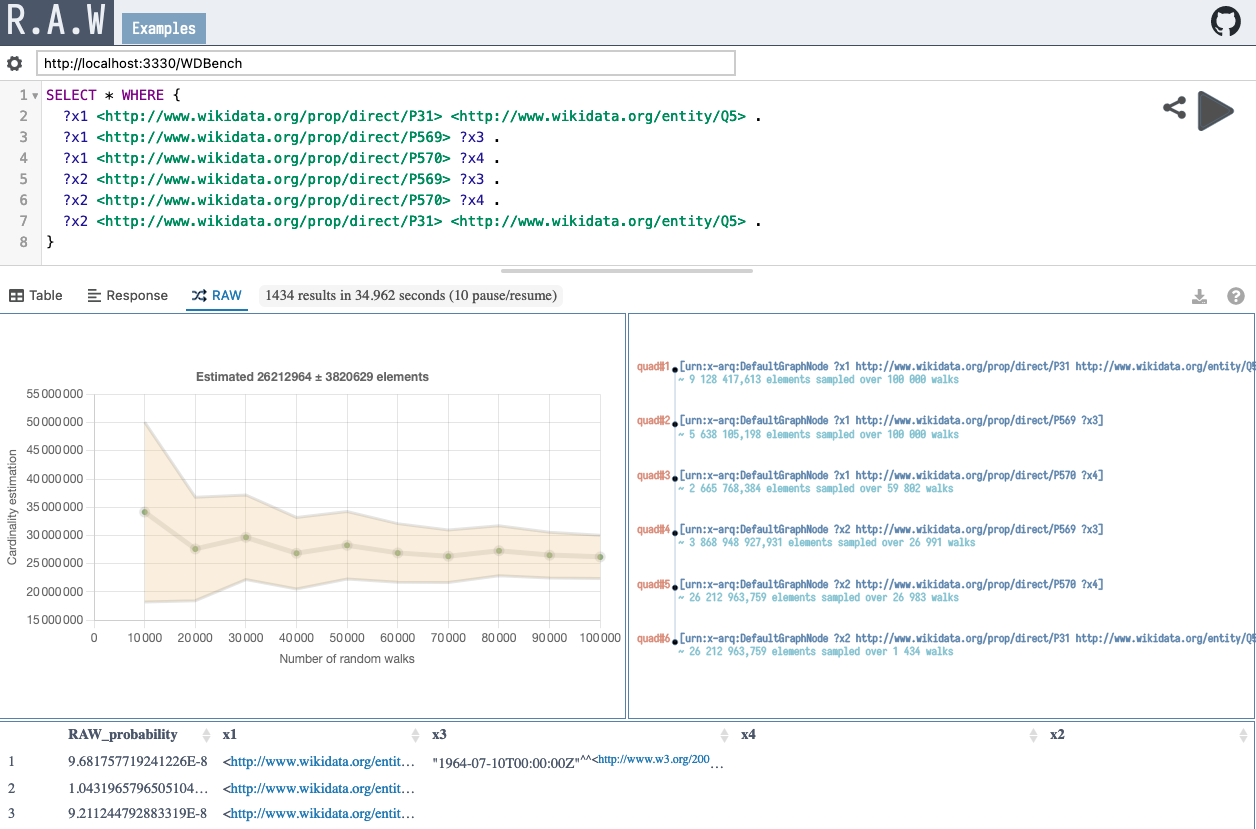
\includegraphics[width=0.85\textwidth]{figures/raw_screenshot.png}
   \caption{\label{fig:raw_screenshot}User interface of \NAME providing useful insights on the query.}
 \end{figure*}

%\paragraph{Target audience.}
%Researchers and practitioners in need of sampling services over RDF
%knowledge graphs. \TODO{In fields.}

 As a motivating example, we rely on the query $Q_{604}$ of
 WDBench~\cite{angles2022wdbench} presented in the
 figure~\ref{fig:raw_screenshot}. This query are looking for people
 with the same birth and death date. This query returns ~25M results,
 time-out on the public Wikidata SPARQL endpoint, and takes more than
 2 hours to execute on JENA. However, using \NAME, in 35 seconds, it
 is possible to estimate that the query should return around 26
 millions of results more or less 3 millions and return 1434 random
 results

 
% \paragraph{Web interface.}
Figure~\ref{fig:raw_screenshot} presents the user interface exploiting
\NAME's random walks. The top part of the figure shows where the users
type their queries. By pressing the play button, it asks the server
for random walks on this whole BGP. When the server reaches a
configurable threshold of $10 000$ random walks, or $60s$ execution
time, it returns its results. By repeating the operation, results are
merged iteratively in a pay-as-you-go fashion hence displaying more
accurate information. Figure~\ref{fig:raw_screenshot} shows that over
$10$ iterations, \NAME performed $100k$ random walks but only $1434$
actual successes.  Yet, the bottom left figure provides an estimation
of the number of results over the number of random walks with
confidence intervals. The bottom right figure provides the estimated
number of intermediate results along with the number of random walks
that reached each triple/quad pattern.  Finally, the bottom part shows
both failed and succeeded random walks along with the probability that
they were chosen at execution time.

% \paragraph{Getting insights on timed out WDBench queries.}
% A few queries of WDBench fail to execute under the 60 seconds mark,
% providing nothing whatsoever. We execute these queries using \NAME and
% show that, with as little as 1 second, we retrieve interesting
% insights on the query plan that may help optimizers to perform their
% join ordering. We also get a rough approximation of the number of
% results that we improve by executing the query for additional seconds.
% The plotted curve converges towards the actual cardinality of the query.



% %%% Local Variables:
% %%% mode: latex
% %%% TeX-master: "../paper.tex"
% %%% End:
